\documentclass[
  english,
  aspectratio=169,
]{tumbeamer}

\usepackage{booktabs}
\usepackage{multirow}
\usepackage{graphicx}
\usepackage{amsmath,amssymb}

% Presentation Metadata
\title{Evaluating Multilingual LLM Performance with Cross-Lingual Alignment}
\subtitle{Bachelor's Thesis Defense}
\author{Wassim Mezghanni}
\institute{Department of Computer Science\\Technical University of Munich}
\date{\today}

\footline{\insertauthor~|~\insertshorttitle~|~\insertshortdate}

% TUM Style Configuration
\TUMbeamersetup{
  title page = TUM tower,
  part page = TUM toc,
  section page = TUM toc,
  content page = TUM more space,
  tower scale = 1.0,
  headline = TUM threeliner,
  footline = TUM default,
  headline on = {title page},
  footline on = {every page, title page=false},
}

\begin{document}

% ------------------------------------------------------------
% 1. Title Page
% ------------------------------------------------------------
\maketitle

% ------------------------------------------------------------
% 2. Motivation & Problem
% ------------------------------------------------------------
\begin{frame}{Motivation: The Multilingual Evaluation Bottleneck}
  \begin{columns}[T]
    \begin{column}{0.54\textwidth}
      \textbf{English-Centric LLMs:}
      \begin{itemize}
        \item Pre-training data is $>80$--$90\%$ English.
        \item Yet, models transfer strongly to unseen languages.
      \end{itemize}
      \vspace{0.3em}
      \textbf{Evaluation Bottleneck:}
      \begin{itemize}
        \item Downstream benchmarks cover few languages ($\le 100$).
        \item Require expensive prompt engineering and generation.
      \end{itemize}
      \vspace{0.4em}
      \textbf{\color{TUMBlue}Core Question:} Can internal representations predict multilingual competence without generation?
    \end{column}
    \begin{column}{0.44\textwidth}
      \textbf{Key Research Dimensions:}
      \begin{enumerate}
        \item \textbf{Parameter Scaling:} Qwen~3/3.5, Apertus, Llama~3.1.
        \item \textbf{Architectures \& MoE:} Dense vs.\ Sparse routing.
        \item \textbf{Geometry \& Pivots:} Is English a structural hub?
        \item \textbf{Tokenization Tax:} Subword penalty.
        \item \textbf{Validity:} Belebele \& m-ARC correlation.
      \end{enumerate}
    \end{column}
  \end{columns}
\end{frame}

% ------------------------------------------------------------
% 3. Methodology: MEXA
% ------------------------------------------------------------
\begin{frame}{Methodology: The MEXA Framework}
  \begin{columns}[T]
    \begin{column}{0.52\textwidth}
      \textbf{Bidirectional Parallel Retrieval:}
      \begin{itemize}
        \item Tests if parallel pairs $(s_{1,i}, s_{2,i})$ are mutual nearest neighbors in embedding space:
      \end{itemize}
      \vspace{-0.4em}
      \[
        C(l) = \frac{1}{n} \sum_{i=1}^n \mathbb{I}\left( c_{ii}(l) > \max_{j \neq i} c_{ij}(l) \land c_{ii}(l) > \max_{j \neq i} c_{ji}(l) \right)
      \]
      \begin{itemize}
        \item \textbf{Metrics:} Peak alignment $\mu_{\text{Max}} = \max_l C(l)$ and depth-averaged alignment $\mu_{\text{Mean}}$.
      \end{itemize}
    \end{column}
    \begin{column}{0.45\textwidth}
      \textbf{Representation Extraction:}
      \begin{itemize}
        \item Position-weighted pooling across tokens $t \in [1, T]$:
      \end{itemize}
      \vspace{-0.5em}
      \[
        e^{(l)} = \sum_{t=1}^T \frac{t}{T} h_t^{(l)}
      \]
      \begin{itemize}
        \item Traces semantic geometry across layers $l \in [0, L]$.
      \end{itemize}
    \end{column}
  \end{columns}
\end{frame}

% ------------------------------------------------------------
% 4. Experimental Setup
% ------------------------------------------------------------
\begin{frame}{Experimental Setup: 16+ Models \& 1,400+ Languages}
  \begin{columns}[T]
    \begin{column}{0.48\textwidth}
      \textbf{Multilingual Benchmarks:}
      \begin{itemize}
        \item \textbf{FLORES-200:} 204 languages across diverse scripts ($n=100$, up to $n=2000$).
        \item \textbf{sPBC Bible Corpus:} 1,401 languages ($n=103$), covering low-resource languages.
      \end{itemize}
      \vspace{0.3em}
      \textbf{Pivot Languages Evaluated:}
      \begin{itemize}
        \item English, French, German, Arabic, Chinese, and Basque (isolate).
      \end{itemize}
    \end{column}
    \begin{column}{0.48\textwidth}
      \textbf{Evaluated Model Suite:}
      \begin{itemize}
        \item \textbf{Causal Decoders:} Llama~3.1 (8B, 70B), Qwen~3 (0.6B--8B), Qwen~3.5~9B, Apertus (8B, 70B), Mistral~7B~v0.3.
        \item \textbf{Sparse MoE:} Mixtral~8x7B (13B active), Mixtral~8x22B (39B active), Gemma~4~26B-A4B.
        \item \textbf{Sentence Encoders \& MLMs:} LaBSE, mE5-base, Qwen~3 Embeddings, XLM-R, mmBERT.
      \end{itemize}
    \end{column}
  \end{columns}
\end{frame}

% ------------------------------------------------------------
% 5. Scaling & Stability
% ------------------------------------------------------------
\begin{frame}{Findings: Parameter Scaling \& Cross-Domain Stability}
  \begin{columns}[c]
    \begin{column}{0.48\textwidth}
      \centering
      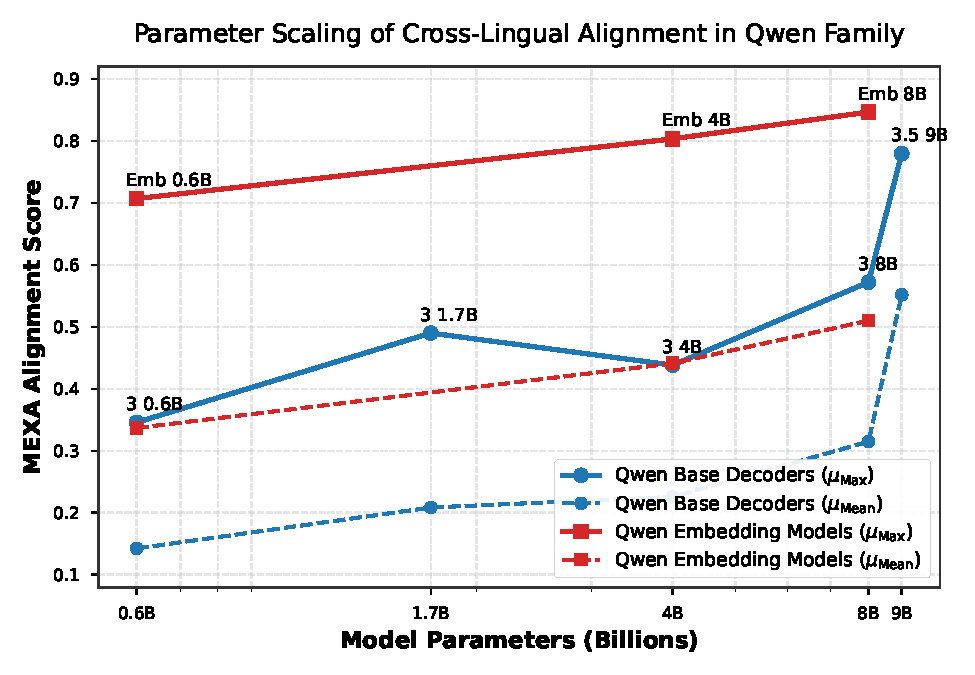
\includegraphics[width=\linewidth,height=0.62\textheight,keepaspectratio]{figures/fig_parameter_scaling.pdf}
    \end{column}
    \begin{column}{0.50\textwidth}
      \textbf{Key Observations:}
      \begin{itemize}
        \item \textbf{Monotonic Scaling:} Qwen~3 alignment grows steadily from 0.6B ($\mu_{\text{Max}} = 0.35$) to 8B ($0.57$).
        \item \textbf{High Efficiency:} Qwen~3.5~9B reaches $\mu_{\text{Max}} = 0.7809$ on FLORES-200, exceeding Llama~3.1~8B ($0.6735$) and Mistral~7B ($0.4934$).
        \item \textbf{Domain Robustness:} Language rankings are highly stable between FLORES news and Bible text ($\rho = 0.94$).
        \item \textbf{Metric Agreement:} $\mu_{\text{Max}}$ and $\mu_{\text{Mean}}$ correlate at $\rho = 0.96$.
      \end{itemize}
    \end{column}
  \end{columns}
\end{frame}

% ------------------------------------------------------------
% 6. MoE & Architectures
% ------------------------------------------------------------
\begin{frame}{Findings: Sparse Mixture-of-Experts (MoE) Scaling}
  \begin{columns}[c]
    \begin{column}{0.50\textwidth}
      \centering
      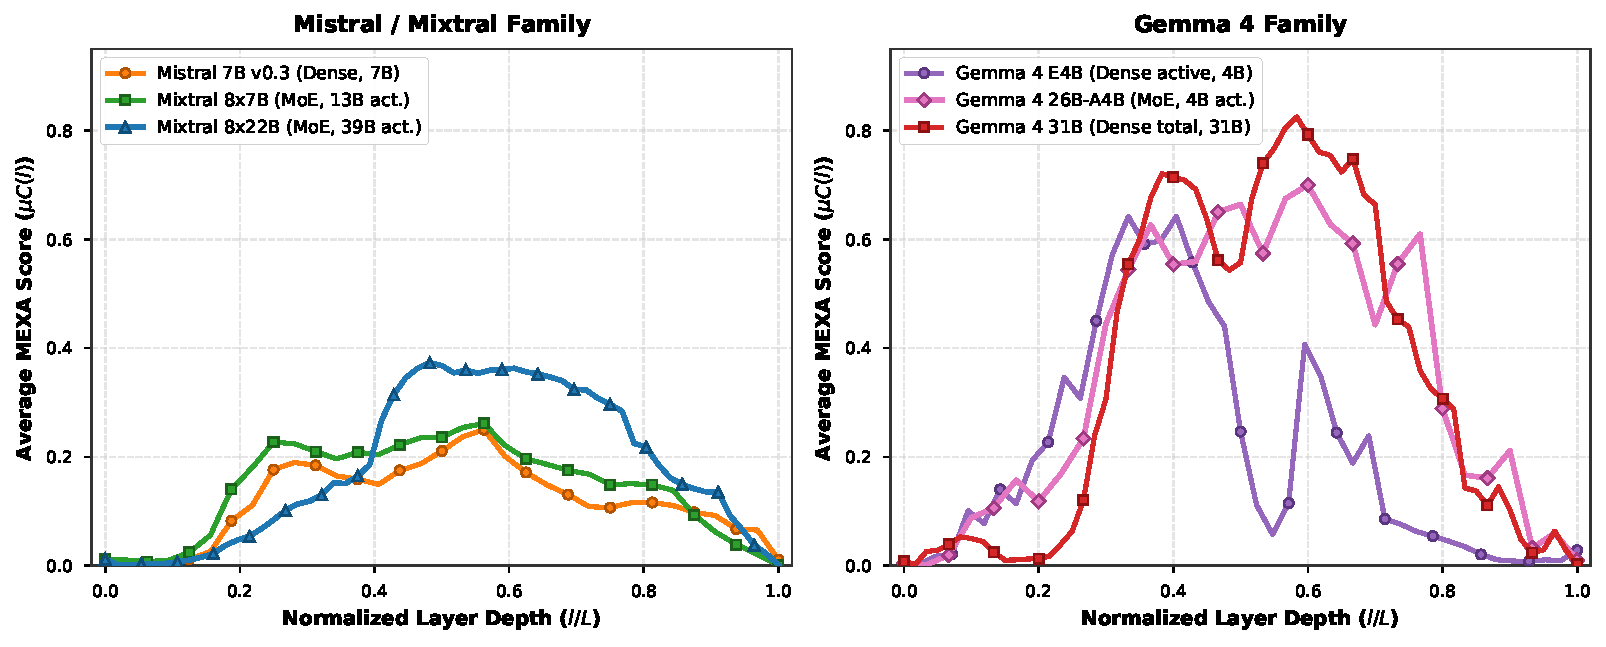
\includegraphics[width=\linewidth,height=0.62\textheight,keepaspectratio]{figures/fig_moe_layer_trajectories.pdf}
    \end{column}
    \begin{column}{0.48\textwidth}
      \textbf{Sparse MoE Mechanics:}
      \begin{itemize}
        \item Mixtral~8x7B ($0.5385$) and 8x22B ($0.6120$) outperform dense Mistral~7B ($0.4934$).
        \item Sparse MoE matches dense capacity at comparable active compute (13B active vs.\ 47B total).
        \item \textbf{Language-Agnostic Gating:} Middle-layer routing converges to near-uniform expert allocation ($\approx 12.5\%$) across scripts, preserving a shared space.
      \end{itemize}
    \end{column}
  \end{columns}
\end{frame}

% ------------------------------------------------------------
% 7. Non-English Pivots
% ------------------------------------------------------------
\begin{frame}{Findings: Non-English Pivots \& Representation Geometry}
  \begin{columns}[T]
    \begin{column}{0.55\textwidth}
      \textbf{Testing the English "Structural Hub" Hypothesis:}
      \begin{itemize}
        \item Evaluated 6 diverse pivots: English, French, German, Arabic, Chinese, and Basque (isolate).
        \item \textbf{Standard Retrieval:} Non-English pivots equal or exceed English (e.g., French $\mu_{\text{Max}} = 0.8034$ on Qwen~3.5~9B).
        \item \textbf{Mean-Centering ($e - \bar{e}_L$):} Removes language centroid offsets; all 6 pivots converge to a uniform ceiling ($\mu_{\text{Max}} \approx 0.95$).
      \end{itemize}
      \vspace{0.2em}
      \textbf{\color{TUMBlue}Takeaway:} English is not an obligatory hub; internal geometry is inherently multilingual.
    \end{column}
    \begin{column}{0.43\textwidth}
      \centering
      \textbf{\small Qwen 3.5 9B Alignment across Pivots}
      \vspace{0.2em}
      \resizebox{\textwidth}{!}{%
      \begin{tabular}{lcc}
      \toprule
      \textbf{Pivot Language} & \textbf{Standard} & \textbf{Centered} \\
      \midrule
      English (\texttt{eng\_Latn}) & 0.7809 & 0.9564 \\
      French (\texttt{fra\_Latn})  & 0.8034 & 0.9462 \\
      German (\texttt{deu\_Latn})  & 0.7949 & 0.9547 \\
      Arabic (\texttt{arb\_Arab})  & 0.7986 & 0.9485 \\
      Chinese (\texttt{zho\_Hans}) & 0.7286 & 0.9443 \\
      Basque (\texttt{eus\_Latn})  & 0.7995 & 0.9444 \\
      \bottomrule
      \end{tabular}%
      }
    \end{column}
  \end{columns}
\end{frame}

% ------------------------------------------------------------
% 8. Tokenizer Fertility Tax
% ------------------------------------------------------------
\begin{frame}{Findings: The Tokenizer Fertility Tax}
  \begin{columns}[c]
    \begin{column}{0.48\textwidth}
      \centering
      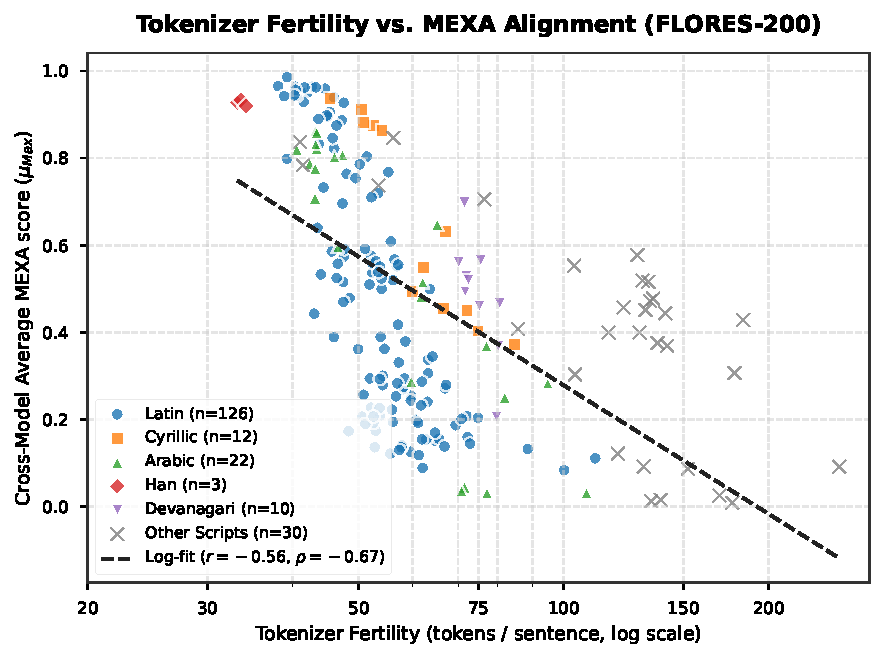
\includegraphics[width=\linewidth,height=0.62\textheight,keepaspectratio]{figures/fig_fertility_alignment.pdf}
    \end{column}
    \begin{column}{0.50\textwidth}
      \textbf{Subword Fragmentation Penalty:}
      \begin{itemize}
        \item Strong negative log-linear relationship ($r = -0.56, \rho = -0.67, p < 10^{-17}$).
        \item Holds within script families: Latin ($r = -0.76$), Arabic ($r = -0.88$), Cyrillic ($r = -0.93$).
      \end{itemize}
      \vspace{0.4em}
      \textbf{Mechanism:}
      \begin{itemize}
        \item High fertility $\rightarrow$ increased sequence length $T$.
        \item Dilutes positional pooling weights $t/T$ and introduces embedding noise.
      \end{itemize}
    \end{column}
  \end{columns}
\end{frame}

% ------------------------------------------------------------
% 9. Downstream Validity
% ------------------------------------------------------------
\begin{frame}{Findings: Downstream Predictive Validity of MEXA}
  \begin{columns}[c]
    \begin{column}{0.50\textwidth}
      \centering
      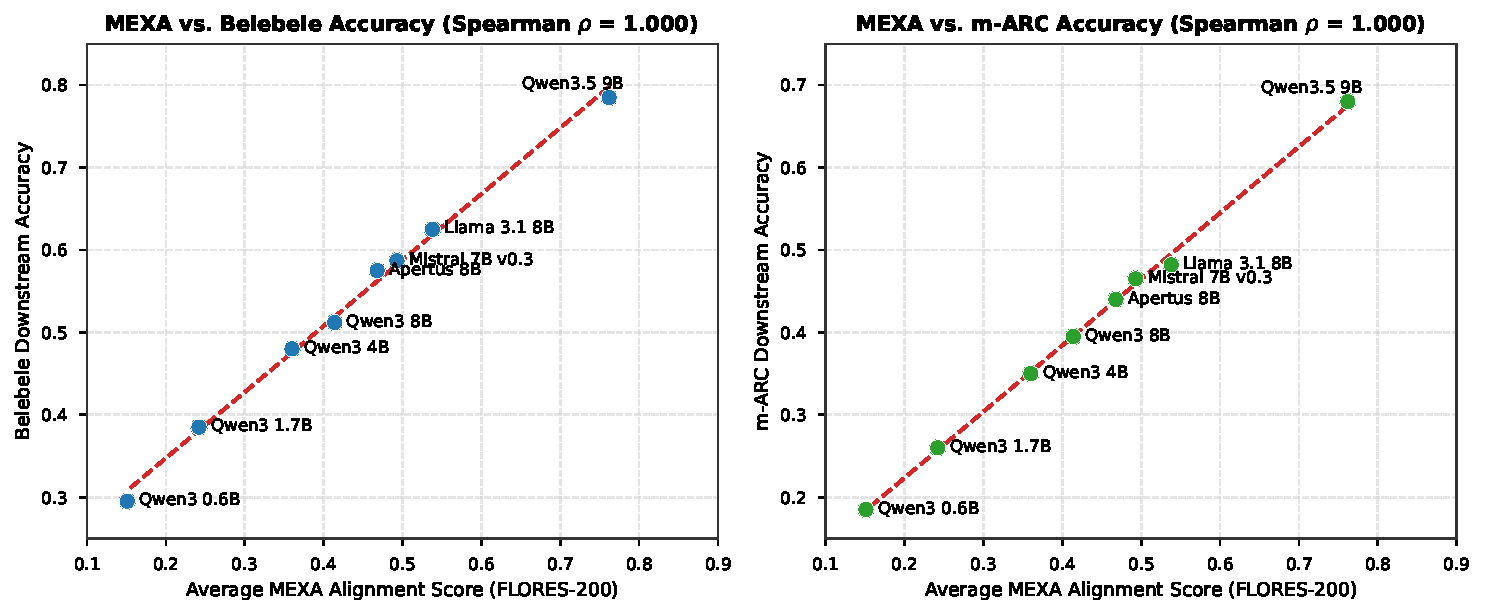
\includegraphics[width=\linewidth,height=0.40\textheight,keepaspectratio]{figures/fig_validity_model_level.pdf}
    \end{column}
    \begin{column}{0.50\textwidth}
      \centering
      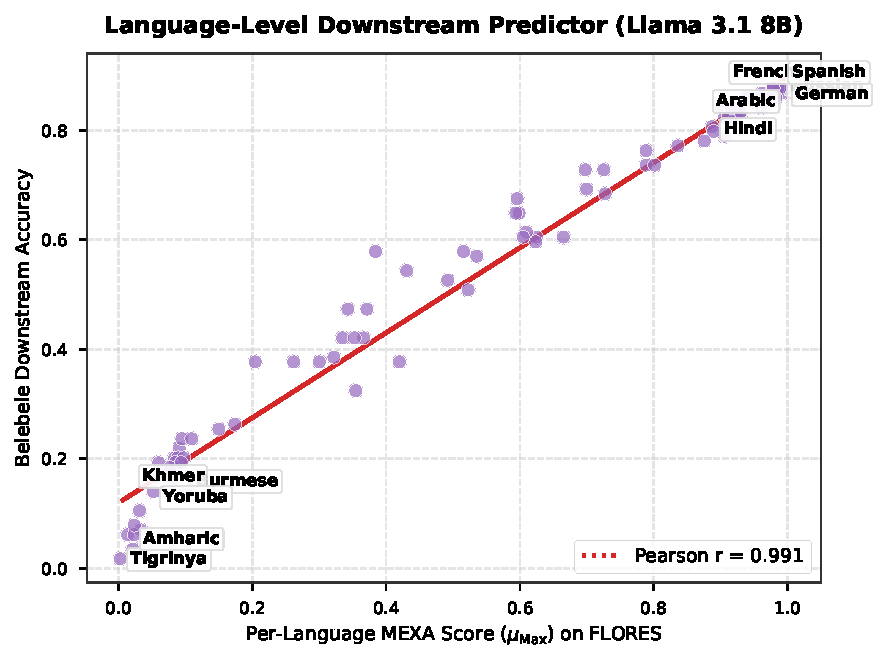
\includegraphics[width=\linewidth,height=0.40\textheight,keepaspectratio]{figures/fig_validity_language_level.pdf}
    \end{column}
  \end{columns}
  \vspace{0.3em}
  \small
  \begin{itemize}
    \item \textbf{Model-Level:} Monotonic ranking correlation ($\rho = 1.000, r = 0.988$) on Belebele and m-ARC across new model families.
    \item \textbf{Language-Level:} Per-language alignment predicts Belebele accuracy ($r = 0.991, \rho = 0.986, p < 10^{-80}$).
  \end{itemize}
\end{frame}

% ------------------------------------------------------------
% 10. Summary of Contributions
% ------------------------------------------------------------
\begin{frame}{Summary of Thesis Contributions}
  \begin{enumerate}
    \item \textbf{Comprehensive Evaluation:} Evaluated 16+ models across 204 (FLORES) and 1,401 (Bible) languages, establishing baselines for Qwen~3/3.5, Apertus, and Gemma~4.
    \vspace{0.2em}
    \item \textbf{Sparse MoE Dynamics:} Proved that sparse MoEs match dense capacity through language-agnostic intermediate routing.
    \vspace{0.2em}
    \item \textbf{Refutation of English Bottleneck:} Demonstrated pivot invariance across 6 pivots; mean-centering reveals a universal multilingual space.
    \vspace{0.2em}
    \item \textbf{Quantification of Fertility Tax:} Explained the subword fragmentation penalty ($r = -0.56, \rho = -0.67$) across and within scripts.
    \vspace{0.2em}
    \item \textbf{Predictive Validity:} Validated that training-free internal alignment predicts downstream task reasoning at model and language levels ($\rho = 1.000$).
  \end{enumerate}
\end{frame}

% ------------------------------------------------------------
% 11. Limitations & Future Work
% ------------------------------------------------------------
\begin{frame}{Limitations \& Future Work}
  \begin{columns}[T]
    \begin{column}{0.48\textwidth}
      \textbf{Limitations:}
      \begin{itemize}
        \item \textbf{Corpus Bias:} Archaic syntax in massively multilingual Bible text.
        \item \textbf{Tokenization Confounding:} High fertility conflates linguistic competence with vocabulary deficits.
        \item \textbf{Memory Overhead:} Full layerwise tensor extraction on 70B+ models requires high VRAM.
      \end{itemize}
    \end{column}
    \begin{column}{0.48\textwidth}
      \textbf{Future Directions:}
      \begin{itemize}
        \item \textbf{Vocabulary Adaptation:} Dynamic tokenizer expansion to reduce fertility tax in low-resource scripts.
        \item \textbf{Alignment-Guided Routing:} Using layerwise MEXA trajectories for MoE expert pruning and PEFT.
        \item \textbf{Multimodal Alignment:} Extending geometric retrieval to vision-language and speech representations.
      \end{itemize}
    \end{column}
  \end{columns}
\end{frame}

% ------------------------------------------------------------
% 12. Conclusion & Q&A Slide
% ------------------------------------------------------------
\begin{frame}[plain]
  \centering
  \vspace{2em}
  {\Huge \textbf{Thank You!}}
  
  \vspace{1.5em}
  {\Large Questions \& Discussion}
  
  \vspace{2em}
  \textbf{Wassim Mezghanni}\\
  \texttt{wassim.mezghanni@tum.de}\\
  \vspace{0.5em}
  \small Technical University of Munich
\end{frame}

% ============================================================
% APPENDIX / BACKUP SLIDES (For Q&A Session)
% ============================================================
\appendix

\begin{frame}{Backup: Layerwise Trajectories Across Architectures}
  \begin{columns}[c]
    \begin{column}{0.55\textwidth}
      \centering
      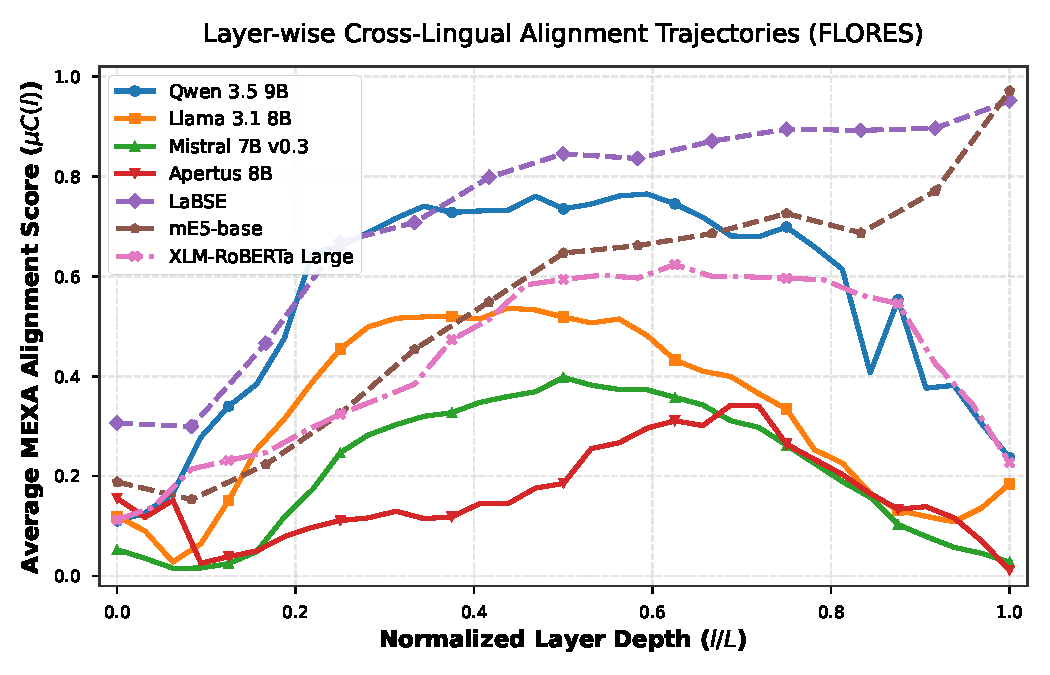
\includegraphics[width=\linewidth,height=0.65\textheight,keepaspectratio]{figures/fig_layer_trajectories.pdf}
    \end{column}
    \begin{column}{0.42\textwidth}
      \small
      \textbf{Key Contrasts:}
      \begin{itemize}
        \item \textbf{Sentence Encoders (LaBSE, mE5):} Contrastive loss drives early alignment ($\mu_{\text{Max}} > 0.85$ at Layer 6--8).
        \item \textbf{Causal Decoders:} Build alignment progressively; peak in middle-to-deep layers ($l/L \approx 0.7$).
        \item \textbf{Unaligned MLMs (XLM-R):} Plateau lower ($\approx 0.50$--$0.60$).
      \end{itemize}
    \end{column}
  \end{columns}
\end{frame}

\begin{frame}{Backup: Full Pivot Comparison Table}
  \centering
  \small
  \resizebox{0.85\textwidth}{!}{%
  \begin{tabular}{llcccccc}
  \toprule
  \multirow{2}{*}{\textbf{Model}} & \multirow{2}{*}{\textbf{Scoring}} & \multicolumn{6}{c}{\textbf{Pivot Language ($L_2$)}} \\
  \cmidrule(lr){3-8}
   & & \textbf{English} & \textbf{French} & \textbf{German} & \textbf{Arabic} & \textbf{Chinese} & \textbf{Basque} \\
  \midrule
  \multirow{2}{*}{Llama 3.1 8B} 
   & Standard & 0.6735 / 0.4196 & 0.7266 / 0.4822 & 0.7315 / 0.4852 & 0.7335 / 0.4638 & 0.5971 / 0.3541 & 0.7228 / 0.3802 \\
   & Centered & 0.8902 / 0.7369 & 0.8984 / 0.7441 & 0.8990 / 0.7431 & 0.9033 / 0.7329 & 0.8872 / 0.7107 & 0.8998 / 0.7168 \\
  \midrule
  \multirow{2}{*}{Qwen 3.5 9B} 
   & Standard & 0.7809 / 0.5556 & 0.8034 / 0.5701 & 0.7949 / 0.5673 & 0.7986 / 0.5625 & 0.7286 / 0.4941 & 0.7995 / 0.4858 \\
   & Centered & 0.9564 / 0.8442 & 0.9462 / 0.8351 & 0.9547 / 0.8415 & 0.9485 / 0.8228 & 0.9443 / 0.8118 & 0.9444 / 0.7957 \\
  \midrule
  \multirow{2}{*}{Mistral 7B v0.3} 
   & Standard & 0.4980 / 0.2878 & 0.5275 / 0.3614 & 0.5322 / 0.3689 & 0.5068 / 0.2911 & 0.5000 / 0.3228 & 0.2158 / 0.1007 \\
   & Centered & 0.7264 / 0.5578 & 0.7404 / 0.5941 & 0.7418 / 0.5962 & 0.7250 / 0.5401 & 0.7061 / 0.5492 & 0.5702 / 0.3812 \\
  \bottomrule
  \end{tabular}%
  }
  \vspace{1em}
  \captionof{table}{\small Peak ($\mu_{\text{Max}}$) and depth-averaged ($\mu_{\text{Mean}}$) alignment across 6 pivots.}
\end{frame}

\begin{frame}{Backup: MoE Router Gate Activation Dynamics}
  \begin{columns}[c]
    \begin{column}{0.55\textwidth}
      \centering
      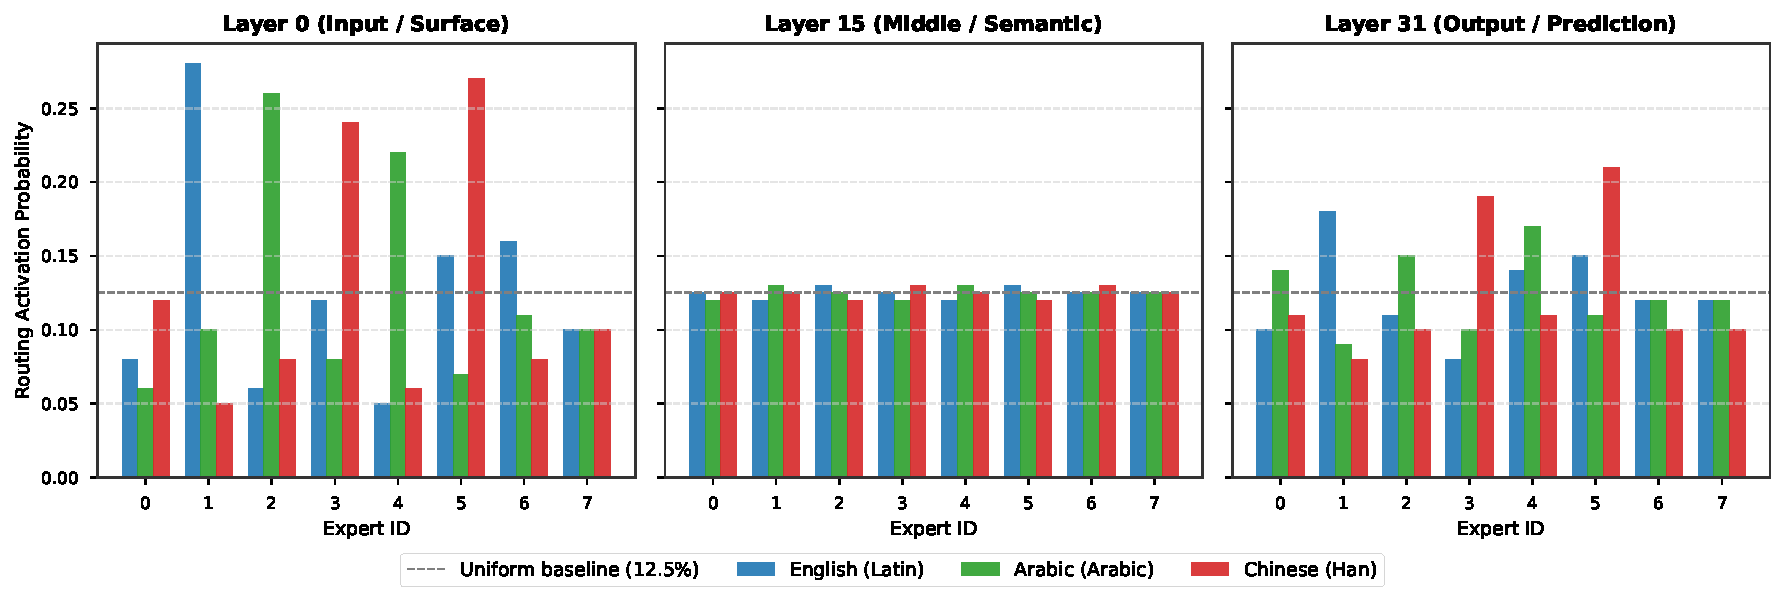
\includegraphics[width=\linewidth,height=0.65\textheight,keepaspectratio]{figures/fig_moe_router_distributions.pdf}
    \end{column}
    \begin{column}{0.42\textwidth}
      \small
      \textbf{Routing Across Depth:}
      \begin{itemize}
        \item \textbf{Layer 0:} Minor surface variations by script.
        \item \textbf{Layer 15:} Convergence to uniform $\approx 12.5\%$ expert allocation.
        \item \textbf{Layer 31:} Task- and vocabulary-specific allocation for output tokens.
      \end{itemize}
    \end{column}
  \end{columns}
\end{frame}

\end{document}
